\documentclass[11pt,  letterpaper]{article}

\usepackage{mathpazo}
\usepackage{fontspec}
\setmainfont{TeX Gyre Pagella}

\input{boilerplate}

\title{Asymmetries in Cricket: The Effects of Winning the Toss on Winning the Match\thanks{This paper incorporates some of the text and results from Sood \& Willis's (2019) working paper: ``Fairly Random: The Impact of Winning the Toss on the Probability of Winning.'' The authors thank Matt Blackwell, Andrew Gelman, Donald Green, Jens Hainmueller, and Daniel Stone for their comments.}}

\author{
Apoorva Lal\thanks{Dept.~of Political Science, Stanford University;  \textsf{apoorval@stanford.edu}.} \;\;
Derek Willis\thanks{News applications developer at ProPublica;  \textsf{dwillis@gmail.com}.}  \;\;
Gaurav Sood\thanks{Independent researcher;  \textsf{gsood07@gmail.com}.} \;\;
Avidit Acharya\thanks{Dept.~of Political Science and Graduate School of Business, Stanford University; \textsf{avidit@stanford.edu}.}
}
\date{\today}


%\usepackage[
%  backend=biber,
%  style=authoryear,
%  citestyle=authoryear,
%  ]{biblatex}
%\addbibresource{biblio.bib}
%\renewbibmacro{in:}{}

\begin{document}

\maketitle

\begin{abstract}

In cricket, which team bats first is determined by a toss. Does the team that wins the toss have an advantage over the other team? We find that, on average, the effect of winning the toss on winning the match is essentially nil in international limited-overs daytime matches but substantial (3.3 percentage points) in day/night matches. In Test cricket, the advantage is even larger (4.9 percentage points). The advantage has exploded in the last decade (to nearly 15 percentage points) after a steady decline. Surprisingly, the effect of the toss does not appear to vary between competitive and non-competitive pairings of teams. And as for the decision to bat or field first, we find the win-loss differential is significantly larger for teams that elect to field; the advantage is negligible among those that elect to bat. Lastly, and perhaps most surprisingly, in rain-delayed matches in which the chasing team's total is adjusted by the Duckworth-Lewis formula, we find that teams that elected to bat first did just as well as those that elected to field first.

\smallskip

\textbf{Key words:} cricket, fairness, randomization

%\textbf{JEL codes:} C72
\end{abstract}



% #### ##    ## ######## ########   #######
%  ##  ###   ##    ##    ##     ## ##     ##
%  ##  ####  ##    ##    ##     ## ##     ##
%  ##  ## ## ##    ##    ########  ##     ##
%  ##  ##  ####    ##    ##   ##   ##     ##
%  ##  ##   ###    ##    ##    ##  ##     ##
% #### ##    ##    ##    ##     ##  #######

\section{Introduction}

In competitive sports, every little thing matters. Nevertheless, many sports leave some key levers out of teams' control and in the hands of fate. In cricket, one such lever---the toss---has been the subject of much attention. In many matches, commentators and cricket enthusiasts claim that there is a definite advantage to either bowling or batting first.\footnote{See, for example, the \href{https://www.quora.com/How-much-does-a-toss-matter-to-a-game-of-cricket}{Quora page on ``How much does a toss matter to a game of cricket?''}} The advantage is also often pointed to by the captains in the pre-toss interview and by the captain of the losing team in the post-match interview. To wrest the advantage, the captain merely needs to pick the side of the coin that will be left facing the sky after the toss and choose whichever one---batting first or batting second---gives the greater advantage. 

In this paper, we measure how well teams have been able to capitalize on any advantage conferred by winning the toss. To answer the question, we collected data on over 35,000 cricket matches across four formats (First Class, ODIs, T20s, and Tests) played over the course of more than one hundred fifty years.

We find that winning the toss increases the chances of winning the match by 1.8 percentage points: toss winners prevail 39.2\% of the time and lose 37.4\% of the time; the rest of the matches are drawn or tied. The effect of winning the toss is the largest in Tests, where it is 4.9 percentage points and the smallest in ODIs and T20s, where it is essentially zero on average. That said, in day/night ODIs and T20s, the effect of winning the toss is 3.3 percentage points; in day-time matches, the effect is a precise zero.

The effect of the toss in ODIs has remained relatively stable since the 1980's when the one-day format first became popular. In Tests, however, the importance of the toss has varied considerably. The effect of winning the toss in Test cricket was a little over five percentage points before 1990. It then dropped to almost 0 from 1990 to 2010. In the last decade, however, it has exploded, averaging 14.5 percentage points. 

Contrary to conventional wisdom, the effect of winning the toss does not vary dramatically across continents, though the toss appears less critical on European and African wickets than elsewhere. The effect on Aussie and Kiwi wickets (3 percentage points) is not substantially different from its effect on South Asian wickets (2.8 percentage points) but is higher than on European and African wickets (1.1 and 0 percentage points respectively).

With this, we turn to the batting first decision. When pitch and weather conditions are hard to read, and it is not obvious that fielding first has a clear advantage, many cricket commentators suggest that batting first is the appropriate choice: get runs on the board, and put the opposing team under psychological pressure by having them chase the target, worrying about ``required run rates,'' etc. We see that the effect of winning the toss on batting first is 13 percentage points. If one team bats, the other team must field, so this translates to saying that among toss winners, 56.5\% of the teams elect to bat, and the remaining 43.5\% choose to field. Thus, compared to the case where teams are randomly assigned to bat, i.e., the case in which the toss has no effect on the batting decision, toss-winning teams bat an excess of 6.5\% of matches. 

However, we find that of the toss winners that elected to bat, only 38.1\% won the match compared to 37.9\% that lost--- a small difference of 0.2 percentage points. On the other hand, of the toss winners that elected to field, 40.8\% won the match compared to 36.9\% that lost--- a larger difference of 3.9 percentage points. This means that 94\% of the 1.8 percentage point effect of winning the toss can be attributed to instances in which the toss winning team elected to field, and only 6\% of the effect can be attributed to the toss winning team electing to bat. This suggests that teams are better able to capitalize on the toss by electing to field when it is advantageous to do so. 

We also look at how the toss advantage breaks down between teams that elected to bat versus those that elected to field within the various subgroups mentioned above and others. Perhaps the most striking result from this analysis for many cricket followers is that there does not appear to be the case that toss winners that elect to bat first do better than those that elect to field first in rain delayed matches where the chasing total is adjusted according to the \citet{duckworth1998} formula. 

Lastly, a caveat about our findings. Our empirical approach estimates the extent to which teams have been able to capitalize on the advantage granted by winning the toss. The toss may matter a lot in principle, but teams may decide poorly. So, when we refer to ``toss effects'' in this paper, we do not refer to whether there is an advantage to winning the toss in principle, whether any such advantage is exploited in practice.

Our results are pertinent to debates about how cricket should be governed. One argument is that since the toss is random, no team is advantaged by the format prior to the toss; and in fact the luck of the toss along with the strategic choice to bat first or second are integral parts of the game--- not very different from the luck of weather affecting the teams differently. 

An alternative argument, however, is that the toss is problematic because it advantages one team over the other even before the first ball is bowled; and care should be taken to mitigate this asymmetry--- for example, by making cricket pitches more durable so that they don't deteriorate so much so that batting on the final day of a test match is miserable. Otherwise, the toss-winning team could exploit this advantage by batting first, reducing the chance that it has to endure this misery. Moreover, the fact that no side is advantaged \emph{ex-ante} if the toss is random is not enough to justify not correcting any asymmetry created by the toss. In fact, the rules of cricket already try to correct the asymmetry between teams that bat first and those that bat second in one particular instance: In rain-delayed one-day matches, the Duckworth-Lewis formula is used to set a new target for the chasing team.\footnote{The argument that no side was advantaged \emph{ex-ante} could have been used to justify not doing any correction in such rain-delayed matches, and simply declaring that the team that batted first won the match because the chasing team was unable to reach its target. But the designers of one-day cricket were clearly unwilling to allow the bad luck of weather to have this much influence on the game. If addressing the misfortunes of weather are important, it may also be important to address the misfortune of losing the toss.} 

For those who take this latter viewpoint, a straightforward policy prescription that comes out of our analysis is that, at least for ODIs, day-night matches should be avoided. In general, when new formats are introduced (such as the recent introduction of T20s) care should be taken to ensure the toss has little effect. The designers of cricket should always consider ways of leveling the playing field for the competing teams starting from the point at which the game really begins--- the moment the first ball is bowled. 

We do not address these optimal design questions in this paper, but our results are relevant to these issues depending on what the designers of cricket seek to optimize. However, at the end of the paper, we propose (and discuss the possible consequences of) a subtle change to the rules governing the toss: Rather than tossing a coin to confer the choice to bat first or second upon the captain of the toss-winning team, umpires may consider simply tossing a coin to determine which team must bat first.


% ########     ###    ########    ###
% ##     ##   ## ##      ##      ## ##
% ##     ##  ##   ##     ##     ##   ##
% ##     ## ##     ##    ##    ##     ##
% ##     ## #########    ##    #########
% ##     ## ##     ##    ##    ##     ##
% ########  ##     ##    ##    ##     ##

\section{Data}

\subsection{Creating the sample}

We obtained data on cricket matches from the ESPNCricinfo website, which covers international and domestic matches, and maintains statistics on a wide variety of matches across formats.\footnote{Information on the matches was downloaded in June 2020 using a purpose-built library available at \href{https://github.com/dwillis/python-espncricinfo}{https://github.com/dwillis/python-espncricinfo}. The data is available at \href{https://github.com/dwillis/cricket-stats}{https://github.com/dwillis/cricket-stats}.} 

We focus on four formats: T20, ODI, Test, and First Class for both men's and women's teams.\footnote{We exclude List A matches that are not ODIs or T20s. These matches are considered a less professional category (with worse data recording) than the formats that we include.} The data are a near census of the relevant population, only excluding scheduled matches that were abandoned without the toss being conducted, and a small number of limited-overs matches in which the minimum number of overs that must be bowled to establish a result were not met.\footnote{In ODIs, for example, each side must bat at least 20 overs for a result to be declared. We have no reason to suspect that the small matches that were excluded because they did not meet this threshold could be biased enough to affect our conclusions. We drop 426 matches recorded as ``no result,'' 3 matches that are recorded as ``abandoned'' or ``canceled,'' and another three that don't record who batted first. The "no result" matches constitute the largest exclusion we make. They appear to be comprised of matches canceled for idiosyncratic reasons, ranging from the \href{https://www.espncricinfo.com/series/shell-tri-series-1991-92-61203/australia-women-vs-england-women-final-66975/full-scorecard}{a team being unable to bat because of the weather} to cancellations because of \href{https://www.espncricinfo.com/series/australia-tour-of-pakistan-1982-83-61392/pakistan-vs-australia-3rd-odi-64196/full-scorecard}{unwanted audience participation}. In all, we drop approximately 0.07\% of matches.}

Our final sample comprises 35,357 cricket matches across four formats played over the last 150 years. We report the distribution of matches over time and by type in Figure \ref{fig:timeseries_decomp}. As the figure shows, the number of matches has exploded over the last two decades, largely due to the introduction of the enormously popular Twenty-20 (T20) format of the game both in international and domestic tournaments. T20 matches constitute over a quarter of all matches played in the last decade.

% subsubsection data_collection (end)

\subsection{Is the toss random?}

Since our analysis rests on the assumption that the coin toss is random, we start by examining this assumption.\footnote{Prior work by \citet{shafqat2015analysis} and \citet{dawson2009bat} conditions on post-treatment variables, whereas we use only the randomization of the toss to identify toss effects.} Is there any evidence that the coin toss is rigged---for example, does the home side enjoy the rub of the green more often? In order to study this, we compare the rates at which home teams, teams that won the toss in their last match, and underdogs (defined as the lower-ranked team whenever rankings are available for both teams) win the toss relative to their opponents. 

To examine whether the toss is rigged, we compute the odds of seeing as many successes in the same number of draws of a sequence of independent Bernoulli random variables with parameter 0.5. For example, home teams have won 50.81\% of tosses in the 6,377 matches for which we have data. The likelihood of tossing a fair coin 6,377 times and getting at least this percentage of heads is 20.1\%. This chance appears low, but not eyebrow-raisingly so. We find that toss wins are even more balanced for teams that won and lost the last toss, and for teams that are underdogs and favorites. Table \ref{table: balance} reports these balance results. 

That said, we do see one potential source of concern. We find that teams that share their nationality with at least two of the three umpires of the match win 51.3\% tosses in the 4,044 international matches for which we have this data. The likelihood of tossing a fair coin 4,044 times and getting at least this share of heads is only 10\%. This number is certainly low enough to raise some eyebrows. That said, the practice of allowing home-team umpires in international matches ended in 1992, and so these issues are less relevant in recent decades which comprise the bulk of our sample. In addition, a rigged toss in favor of the home team would bias estimates of the advantage of winning the coin toss to the extent that it is correlated with ability. If stronger teams win more tosses, estimates of the advantage of the coin toss would be inflated upwards. And vice versa, if otherwise. Given home teams win more matches and are seen as 'stronger' at home, it is possible that the results are slightly biased upwards. We investigate this point later in the paper, looking at effects post 1992. For now, we proceed as if the toss was random.


% ########  #######   ######   ######
%    ##    ##     ## ##    ## ##    ##
%    ##    ##     ## ##       ##
%    ##    ##     ##  ######   ######
%    ##    ##     ##       ##       ##
%    ##    ##     ## ##    ## ##    ##
%    ##     #######   ######   ######


\section{Do teams exploit the advantage of winning the toss?}

To estimate the advantage of winning the toss, we run regressions on a team $\times$ match level dataset. Let $i$ index teams, and $j$ index matches. $Y_{ij}$ is a dummy for team $i$ winning match $j$, and takes a value of $0.5$ for draws. $Z_{ij}$ is a dummy for team $i$ winning the toss in match $j$. For the main specifications of interest, we estimate regression equations of the form

\begin{equation}\label{eqn:reduced_form}
Y_{ij} = \alpha_0 + \tau Z_{ij} + \gamma_i + \delta_t + \psi_k + \varepsilon_{ij}
\end{equation}

which include fixed effects for teams $\gamma_i$, time $\delta_t$, and match-type $\psi_k$. We cluster the standard errors at the match level.

We report results in Table \ref{table:reduced_form}. We progressively introduce team, match-type, and time period fixed effects in columns 2, 3, and 4, and find that results are remarkably stable. The first column gives the baseline estimate of the toss effect. The 1.8 percentage points difference reflects the fact that toss winners win 39.2\% of the time and lose 37.4\% of the time; the remaining matches are drawn. The estimated effect remains at 1.7 percentage points when we progressively add various fixed effects.

We then proceed to examine the effect of the toss within various subgroups. We report the estimates graphically in Figures \ref{fig:rf_het_TE} - 4 with point estimates and sample sizes as annotations. We summarize the results below:

\textbf{Format.} Toss effects are most pronounced in Test matches followed by first class matches, and are statistically indistinguishable from zero in ODIs and T20s. We estimate the effect of the toss on winning a Test match to be 4.7 percentage points. The effect of the toss in first class matches is 2.3 percentage points. These results support the conventional wisdom among lay cricket followers that the toss grants the greatest advantage in multi-day affairs. Pitches invariably deteriorate over the course of these matches, and the fourth innings in a Test match is often the most challenging time to bat. The pitch deteriorates far less over the course of a day, or in the case of T20s, a few hours. Our null results for limited over matches also extend \citet{de1998winning}, who, based on analysis of data from 427 international one-day matches conclude that ``winning the toss at the outset of a match provides no competitive advantage.''

\textbf{International vs.~Domestic matches.} Toss effects are virtually the same for international and domestic matches (point estimates are 1.7 percentage points in the former, and 1.9 percentage points in the latter). 

\textbf{Effects over time.} Toss effects appear to have declined over time from a high of 9.9 percentage points in the second half of the 19th century to 1.4 percentage points in the last decade. This trend may be a result of a changing composition of matches so we also looked at these trends within formats. T20s have not been played long enough for us to draw any conclusions about how toss effects have changed over time. But within the other formats, we find that toss effects follow a similar pattern, except that in Test cricket there is a peculiar uptick in the last decade: the toss effect jumps from 0 in the decade before to 14.5 percentage points now. We investigate potential sources of the ecological decline below but there are some factors that could be important drivers but for which we do not have the data. For example, cricketers may have become fitter, and able to play for longer periods without tiring as much as they once did, reducing the impact of the order in which they ball or bat. Pitches may have become more resilient to wear than they once were. Teams may have become better informed about how to play more effectively whether they bat first or second, etc. 

\textbf{Relative strength.} We expect the toss to be less important in matches where one team is clearly stronger than the other. We expect the stronger team to win, whether it bats first or second. To test this hypothesis, we use team ranking data published by cricket's official governing body, the International Cricket Council (ICC). The median match is played between teams where the ICC rating difference is 17 points. We use that as the approximate splitting point, splitting the matches into teams where the gap in the ICC ratings of the two teams is less than 15 points and where it is more. In this case, we believe the standard errors are too large for us to arrive at any substantively meaningful conclusions. Statistically, we believe effects larger than 8\% are unlikely. 

\textbf{Continents.} Toss effects vary only somewhat across continents, hovering around 2.5 percentage points for matches played in Asia, Oceania, and the Americas (though the estimates for the Americas are noisier in part due to the smaller number of matches played there). In Europe (effectively England) the toss effect is only 1.1 percentage points (though we cannot rule out a null effect), and in Africa it is essentially zero. Overall, despite there being much talk about the different kinds of wickets across the world, with wickets in certain regions being drier, or stickier, or subject to more wear, these differences do not seem to translate into substantial toss effect differences at least when we look at coarse geographic averages.

\textbf{Day/Night matches.} It is often claimed that the toss is more crucial in day-and-night matches. We find some evidence for this. In the limited overs formats where day/night matches take place (ODIs and T20s), the advantage of winning the toss in a day/night match is 3.3 percentage points, whereas the

advantage of winning the toss in a limited overs match played during the day is zero. 

\textbf{Seasonality.} Weather is also thought to have a large impact on the playing conditions in cricket. Cool overcast weather, for example, is thought to aid swing bowling, especially on English pitches. More generally, the advantage of winning the toss likely varies by weather. Although we do not have data on the weather, we can proxy it with seasons. In particular, students of the game suspect that the advantage of winning the toss in the early English season is especially significant. There is some evidence of a seasonal pattern for matches played in England, with the advantage of winning the toss growing over the summer, though the trend is weak and broken in the month of July.

\textbf{Rain delays.} Finally, we look at the differential effects of winning the toss in ODI matches that were rain-delayed, causing the number of overs bowled in the second innings to be adjusted down. We examine the subset of matches where rain-delays result in revised targets computed using the \citet{duckworth1998} method. This method has been the subject of much controversy, with many cricket fans suggesting that it is rigged against the chasing team. To our surprise, we find no evidence that toss winners are able to exploit the possibility of second-inning rain delays to their advantage. If anything, we see that the toss-winner has a \emph{disadvantage} of 2.4 percentage points in matches subject to the Duckworth-Lewis adjustment, though this point estimate is statistically indistinguishable from zero.\footnote{Toss-winners won 160 out of 333 ODIs with the Duckworth-Lewis adjustment (i.e.~48\%) and 3085 out of 6187 ODIs without the Duckworth-Lewis adjustment (49.9\%).} This, however, does not mean that the Duckworth-Lewis method is not rigged against the chasing team; that issue will be discussed further in the next section.

% subsubsection heterogeneous_treatment_effects (end)

% ########     ###    ########
% ##     ##   ## ##      ##
% ##     ##  ##   ##     ##
% ########  ##     ##    ##
% ##     ## #########    ##
% ##     ## ##     ##    ##
% ########  ##     ##    ##


\section{Batting versus Fielding First}

56.5\% of teams that won the toss elected to bat. This is not surprising given the conventional wisdom is that when you are not sure about whether to bat or field first, bat first. The first column of Table \ref{table:iv_table} shows that 49.2\% of teams that batted first won the match, while 50.8\% of teams that fielded first won. The second column shows that among teams that won the toss and batted first, the ``win-loss differential'' is small: these teams won only 0.2 percentage points more frequently than they lost, winning 38.1\% of matches and losing 37.9\% of matches, as reported in the introduction. This win-loss differential is smaller than it is for teams that won the toss and elected to field. The third column of the table shows that these teams won 3.9 percentage points more frequently than they lost: they won 40.8\% of their matches and lost 36.9\% of them. Combining this information with the fact that 56.5\% of teams that won the toss elected to bat (and only 43.5\% elected to field, as implied by the fourth column of the table), we learn that 94\% ($= .435 \times .039/.018$) of the 1.8 percentage point advantage to winning the toss that we reported in the previous section can be attributed to the success of toss-winning teams that elected to field. To further understand what explains the preference to bat or bowl first, we see how winning the toss affects the choice in various subsets:

\textbf{Format.} Teams appear to have a strong preference for batting first in longer match formats. In Test matches 72.8\% of teams that win the toss elected to bat, whereas in T20s and ODIs this share is only about 52.9\%. In first-class matches it is 56.9\%. 

\textbf{International vs. Domestic matches.} We see no big differences in the propensity to elect to bat first across international versus domestic matches.

\textbf{Effects over time.} Historically, toss-winning teams tilted heavily in favor of batting first, but this declined over the course of the 20th century, and now they show no preference (on average) to bat first. Even for test matches, toss-winning teams tend to be tilting less toward batting first than they once did. Pre-1950, more than 90\% of the teams that won the toss elected to bat, whereas in the last two decades that number is closer to two-thirds. Perhaps players have gotten fitter and are willing to trade off expecting to have to bat on the final day of the match in favor of taking advantage of playing conditions that are favorable to fielding first. As for ODIs, teams interestingly heavily preferred fielding first in the early decades of the format, but in the last thirty years, they have tilted more towards batting first, with just over half of the toss-winning teams electing to bat.

\textbf{Relative strength.} We see no notable differences in the toss-winning captain's choice to bat first across matches that are lopsided and those in which the teams are more evenly matched. This is especially true in Tests but also appears to be true in ODIs, though a slightly larger share of toss-winning teams elect to bat in matches that are lopsided (54.6\%) in comparison to ones that are less lopsided (51.9\%).

\textbf{Continents.} Toss-winning captains show a preference to bat first in matches played in Oceania and Europe, more so than on other pitches. For example, in Europe (mainly England) $64.9\%$ of toss-winning teams elect to bat, and in Oceania, this number is $59.9\%$. By contrast, on Asian wickets, it is only $50.1\%$.

\textbf{Day/Night matches.} The ball being harder to see at night afflicts both batting and fielding. But the difficulty for batsmen is probably greater than it is for fielders. Indeed, within the shorter formats, the variation between day matches and day/night matches is greatest when it comes to the choice to bat first. In day/night matches, $59\%$ of toss-winning teams elect to bat first, whereas in day matches just about half of them do.

\textbf{Seasonality.} The preference to bat first in England follows a broadly similar trend to the toss effect over the course of the year-- rising steadily over the summer, and dropping in September. At its peak in August, top-winning captains choose to bat first $71.9\%$ of the time. At its lowest in April, the  teams that win the toss choose to bat $57.4\%$ of the time.

\textbf{Rain delays.} Remarkably, there is an overall preference to field first in matches that ended up using the Duckworth-Lewis adjustment: only $43.5\%$ of toss-winning teams elected to bat in these matches. If captains have the ability to predict rain (and other) delays, they seem to prefer to bat fewer overs and chase the adjusted target.

\subsection{The Difficulty in Estimating the Advantage to Electing to Bat/Field First}

Despite having reported the `reduced form' and `first stage' effects of the toss, we cannot interpret the ratio of these effects as the causal effect of batting first. If we used the toss as an instrument for batting first, say, we could at best hope to estimate the local average treatment effect (LATE) of electing to bat on winning the match \citep{angrist1996identification}. This is because in our setting treatment effects likely vary across groups: some teams in some circumstances will be better able to capitalize on the ability to bat or field first.  

However, even the conditions under which the LATE is known to be identified are not satisfied in our setting. To see why, first note that our setting has two-sided noncompliance: there are teams that win the toss that bat first, and those that lose the toss that bat first as well. Then, recall that under two-sided noncompliance, the LATE is identified under a monotonicity assumption that rules out defiers. However, defiers are likely to be present in our setting: they correspond to dyads of opposing teams that walk on to the pitch intending to field first if they win the toss. In such a setting, the team that wins the toss will choose to field first and the team that loses the toss will be compelled to bat first. If these defiers are present, which they likely are, the monotonicity assumption does not hold, so we cannot assert that the IV estimates are giving us the LATE.

We make these points more concrete. Recall that we saw that 56.5\% of teams that won the toss elect to bat, which is 6.5 percentage points more than what you would expect if the toss had no effect on the batting/fielding decision. In addition, the reduced form estimated effect of winning the toss on winning the match was 1.8 percentage points, implying that toss winners win an excess of 0.9 percent of matches over parity. The instrumented effect of batting first would then be estimated as 0.9/6.5 = 13.9 percentage points.\footnote{Since the choice to field first is the perfectly colinear inverse of the choice to bat first, flipping the sing of this number gives the estimated instrumented effect of electing to field first.} Can we interpret this as the average rate at which the complier teams that won the toss and elected to bat generated the excess wins? No, because these excess wins could have been generated by the defiers making good decisions to field. Since we saw that teams that win the toss and elect to field first have a higher win-loss differential than those that elect to bat first, it would be irresponsible to rule out this possibility. Consequently, it is unlikely the LATE can be identified in our setting.

\section{Conclusion}

When the toss is unimportant, the game is fair: neither the batting side nor the fielding side has an advantage derived simply from the luck of the toss prior to the first ball being bowled. The toss appears to be unimportant in some settings, but important in others, like day/night matches. 

We end with a small but potentially important policy proposal that cricket boards might consider. We propose auctioning off the ability to choose whether to bat or bowl first. Ask teams to use their knowledge and experience to price the value of getting to pick whether to bowl or bat first. We propose giving teams the time to inspect the playing surface and then asking the teams to place bids for how many runs should be added to the other team's total. The team with the higher bid wins the right to choose whether to bowl or bat. (If the bids are tied, which suggests that teams price the ability to choose the same, an actual coin toss can be used to decide which team chooses and the runs would be added to the other team's score.) Such ways of resolving who has the right to make the choice to bat or field first could make games more competitive, and thus more enjoyable to many viewers. Cricket could benefit from our willingness think outside the box.

\newpage

\bibliography{biblio.bib}

\clearpage


\begin{figure}[tbh]
  \centering
  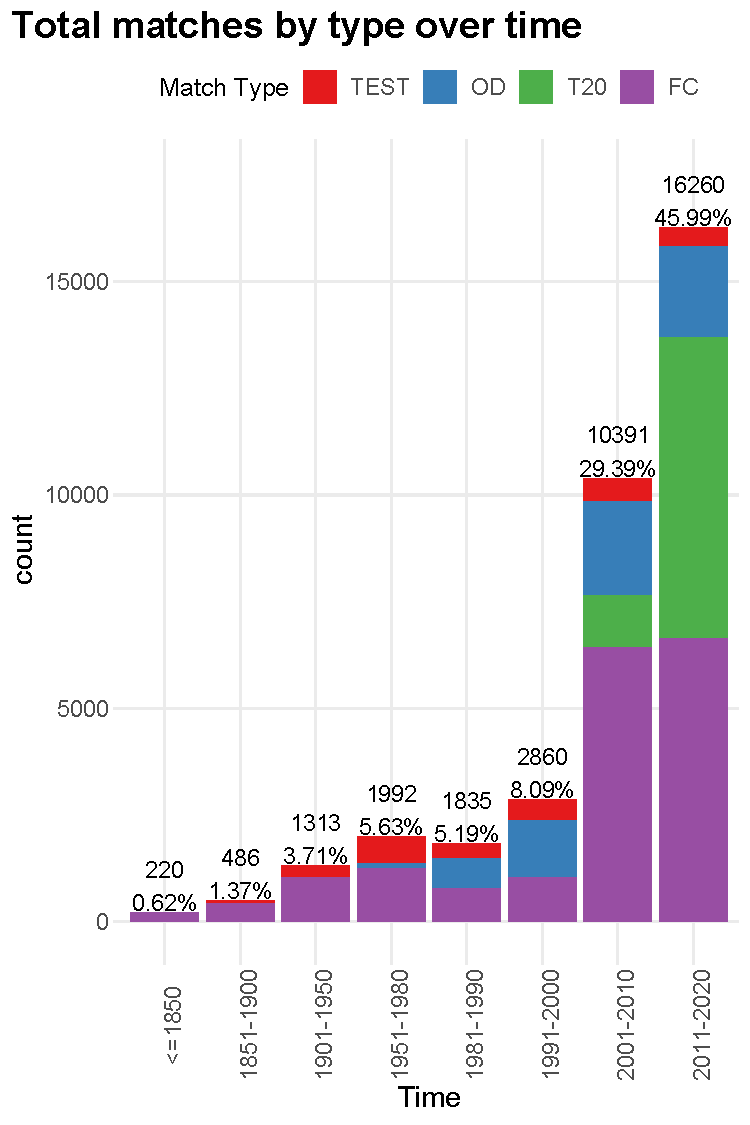
\includegraphics[width=0.6\textwidth,keepaspectratio]{output/matchcounts.pdf}
  \caption{Number of matches by format over time}
  \label{fig:timeseries_decomp}
\end{figure}


\begin{table}[b!]\centering
\begin{tabular}{llll}
 & Toss Wins & Matches & $p$ value\\ \hline
Home team & 3240 & 6377 & 0.201\\
Last toss winners & 17189 & 34283 & 0.611\\
Underdog & 2001 & 4054 & 0.423\\
Home Umpire &  2075	& 4044	& 0.098 \\
\end{tabular}
\caption{Balance \label{table: balance}}
\end{table}


% \clearpage

\begin{table}
\centering
\caption{Reduced Form Effect of Toss on win probability}

\begin{tabular}{@{\extracolsep{5pt}}lcccc} 
\\[-1.8ex]\hline \\[-1.8ex] 
\\[-1.8ex] & (1) & (2) & (3) & (4)\\ 
\hline \\[-1.8ex] 
 Win Toss & 0.018$^{***}$ & 0.017$^{***}$ & 0.017$^{***}$ & 0.017$^{***}$ \\ 
  & (0.005) & (0.005) & (0.005) & (0.004) \\ 
  Constant & 0.491$^{***}$ &  &  &  \\ 
  & (0.002) &  &  &  \\ 
 Team FE &  & $\checkmark$ & $\checkmark$ & $\checkmark$ \\ 
Match-Type FE &  &  & $\checkmark$ & $\checkmark$ \\ 
Time FE &  &  &  & $\checkmark$ \\ 
\hline &  &  &  &  \\ 
Number of Matches & 35357 & 35357 & 35357 & 35357 \\ 
\hline \\[-1.8ex] 
\end{tabular} 

\label{table:reduced_form}
\end{table}

\begin{figure}[b]
  \centering
  \figinc{output/reduced_form_by_matchtype.pdf}
  \caption{Effect of winning the toss on win probability decomposed across different match types, over time, and by continent.}
  \label{fig:rf_het_TE}
\end{figure}

% \clearpage

\begin{figure}[b]
  \centering
  \figinc{output/reduced_form_by_format_overtime.pdf}
  \caption{Effect of winning the toss on win probability decomposed by format over time}
  \label{fig:rf_het_TE2}
\end{figure}

\begin{figure}[b]
  \centering
  \figinc{output/reduced_form_by_rank_dl_season.pdf}
  \caption{Effect of winning the toss on win probability decomposed by competitiveness, use of DL, and Seasonality}
  \label{fig:rf_het_TE3}
\end{figure}

\clearpage

\begin{table}
\scriptsize
\centering
\caption{Batting first and win probability}

\begin{tabular}{@{\extracolsep{5pt}}lccccccc} 
\\[-1.8ex]\hline \\[-1.8ex] 
 & \multicolumn{3}{c}{OLS} & First-Stage & \multicolumn{3}{c}{IV} \\ 
\\[-1.8ex] & (1) & (2) & (3) & (4) & (5) & (6) & (7)\\ 
\hline \\[-1.8ex] 
 Bat First & $-$0.016$^{***}$ & 0.002 & $-$0.039$^{***}$ &  &  &  &  \\ 
  & (0.005) & (0.006) & (0.007) &  &  &  &  \\ 
  Win Toss &  &  &  & 0.130$^{***}$ &  &  &  \\ 
  &  &  &  & (0.005) &  &  &  \\ 
  Bat First (IV) &  &  &  &  & 0.139$^{***}$ & 0.134$^{***}$ & 0.134$^{***}$ \\ 
  &  &  &  &  & (0.036) & (0.036) & (0.036) \\ 
  Constant & 0.508$^{***}$ & 0.499$^{***}$ & 0.519$^{***}$ & 0.435$^{***}$ & 0.430$^{***}$ &  &  \\ 
  & (0.002) & (0.003) & (0.004) & (0.003) & (0.018) &  &  \\ 
 Sample & All & TW bats & TW fields & All & All & All & All \\ 
FS F-Stat &  &  &  &  &  & 604.71 & 579.95 \\ 
Team FE &  &  &  &  &  & $\checkmark$ & $\checkmark$ \\ 
Match-Type FE &  &  &  &  &  & $\checkmark$ & $\checkmark$ \\ 
Decade FE &  &  &  &  &  &  & $\checkmark$ \\ 
\hline &  &  &  &  &  &  &  \\ 
Number of Matches & 35357 & 19971 & 15386 & 35357 & 35357 & 35357 & 35357 \\ 
\hline \\[-1.8ex] 
\end{tabular} 

\label{table:iv_table}
\end{table}


\begin{figure}
 \centering
 \figinc{output/first_stage_by_matchtype.pdf}
 \caption{Toss effects on choice to bat decomposed across different match
 types, timing, and continent.}
 \label{fig:fs_het_TE1}
\end{figure}

\begin{figure}
 \centering
 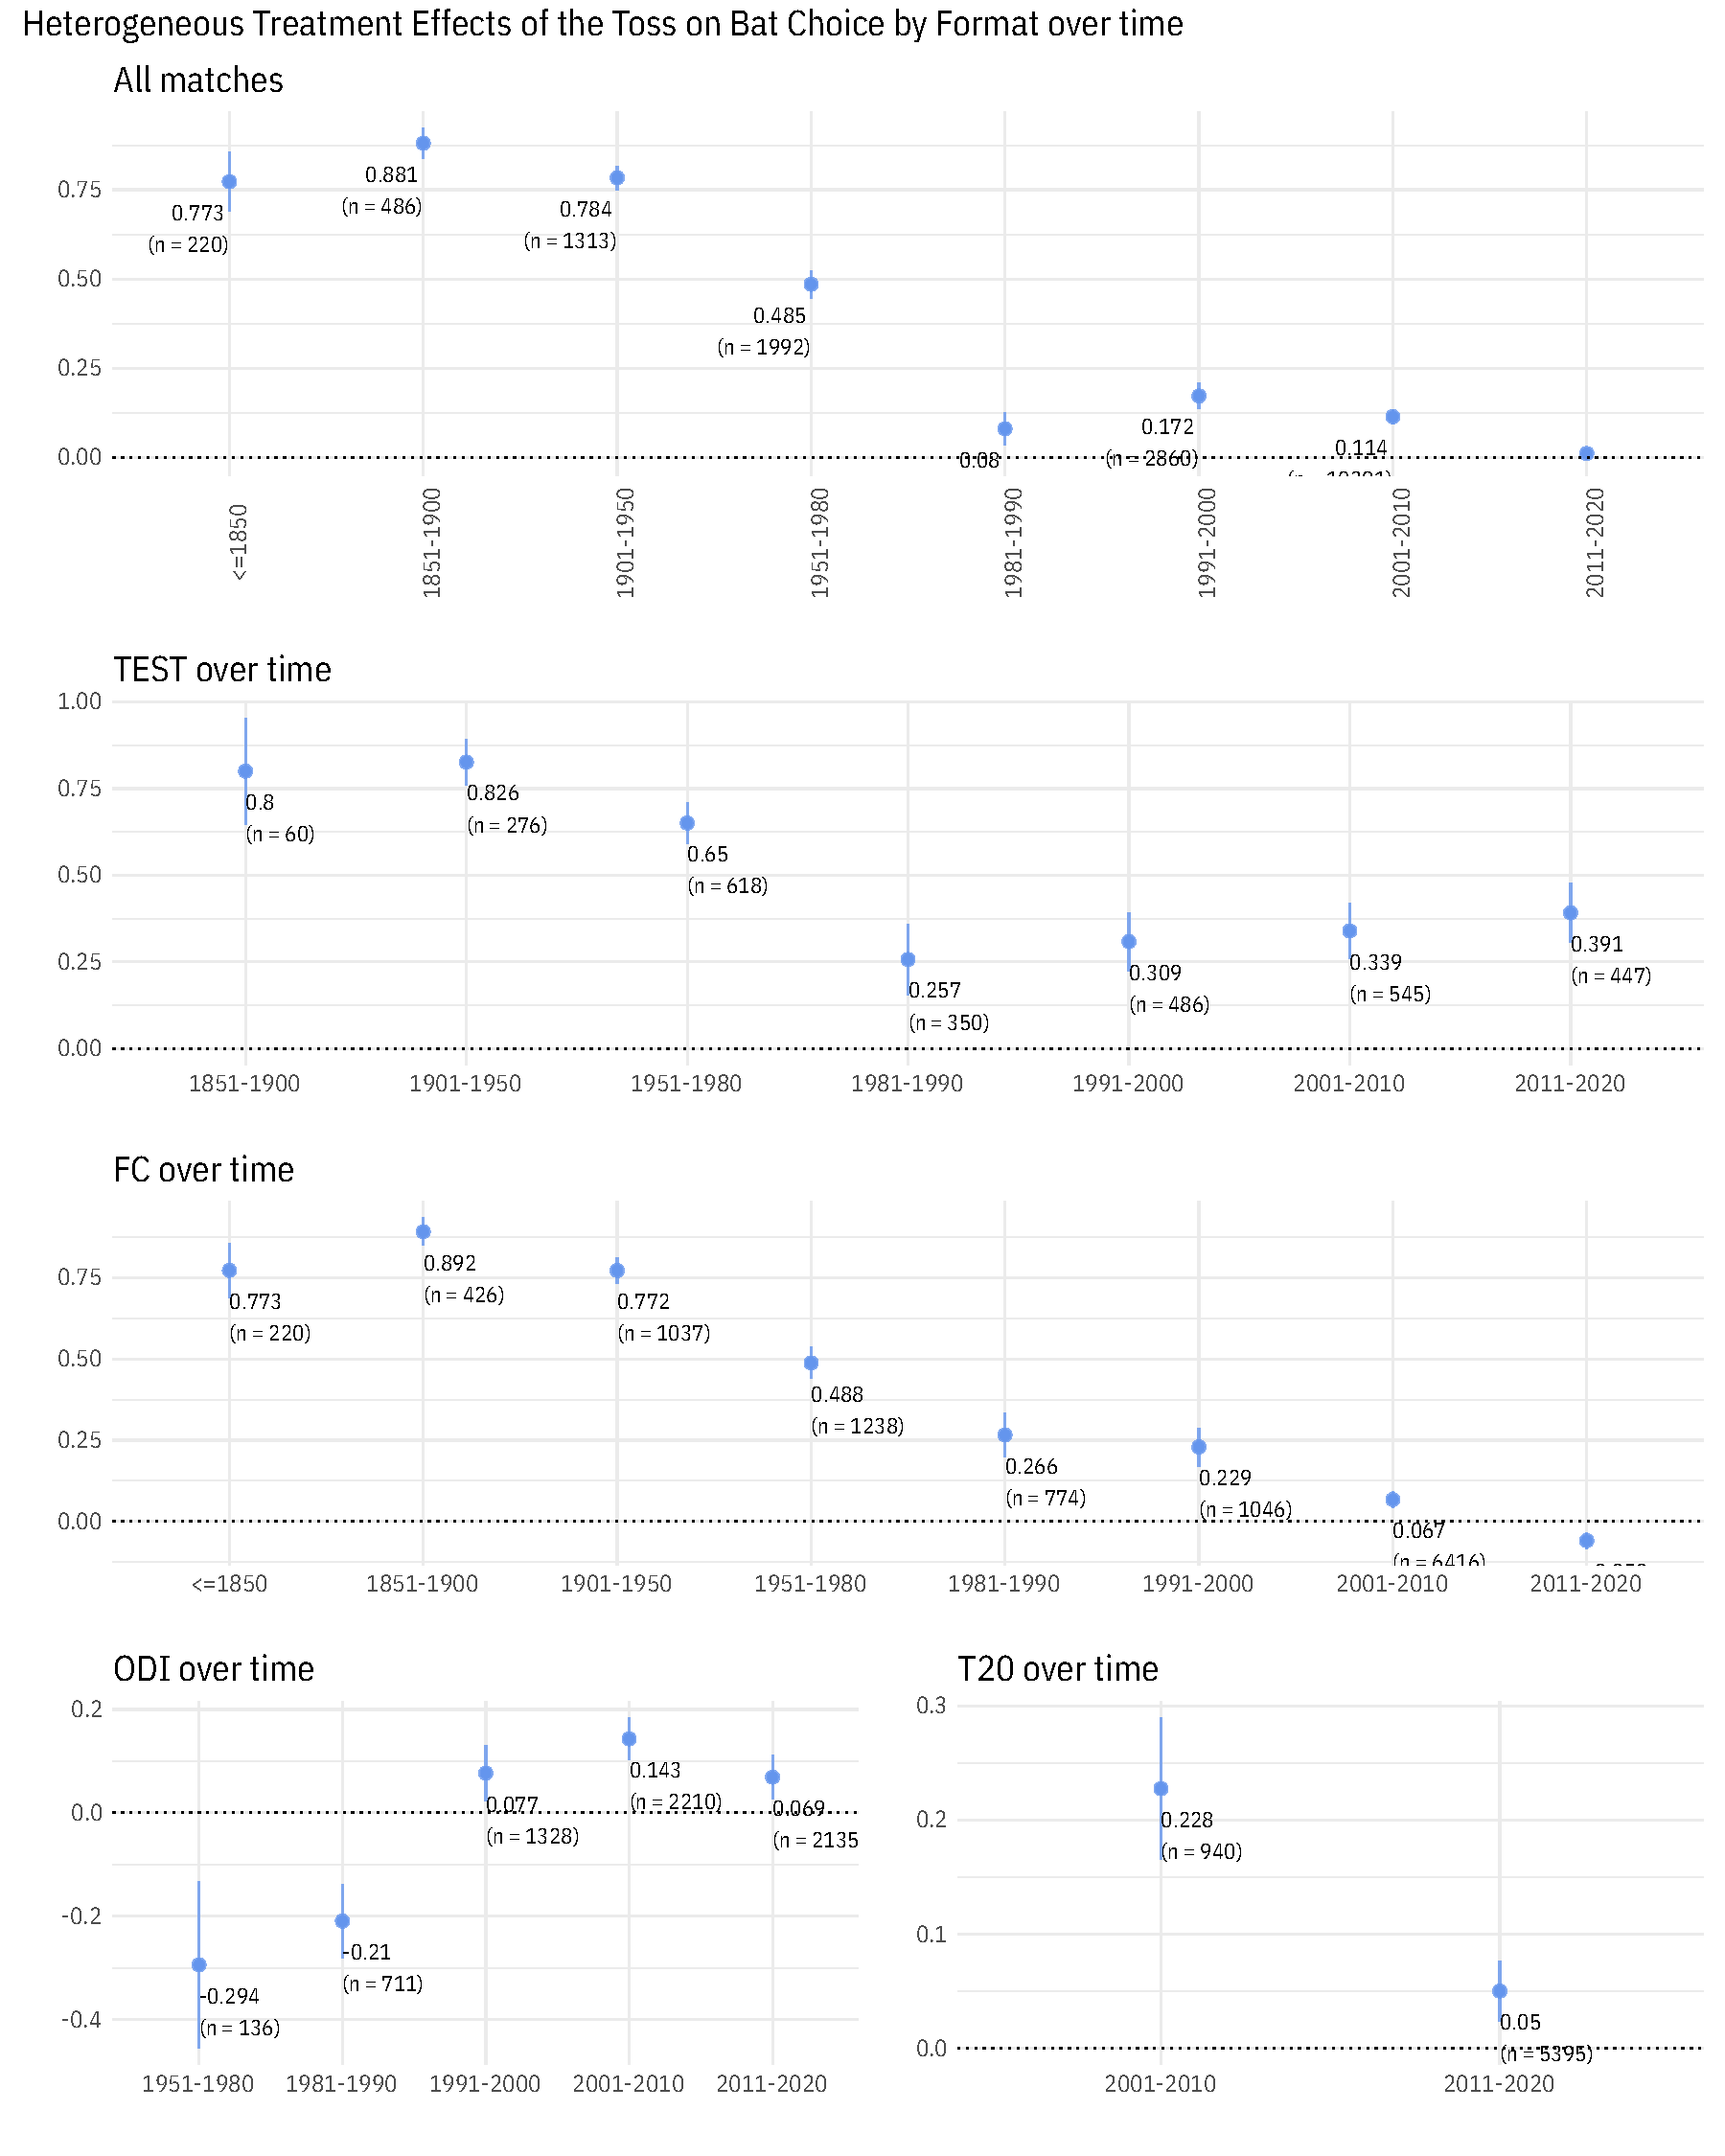
\includegraphics[width=\textwidth,keepaspectratio]{output/first_stage_by_format_overtime.pdf}
 \caption{Toss effects on choice to bat decomposed across different formats
 over time}
 \label{fig:fs_het_TE2}
\end{figure}


\begin{figure}
 \centering
 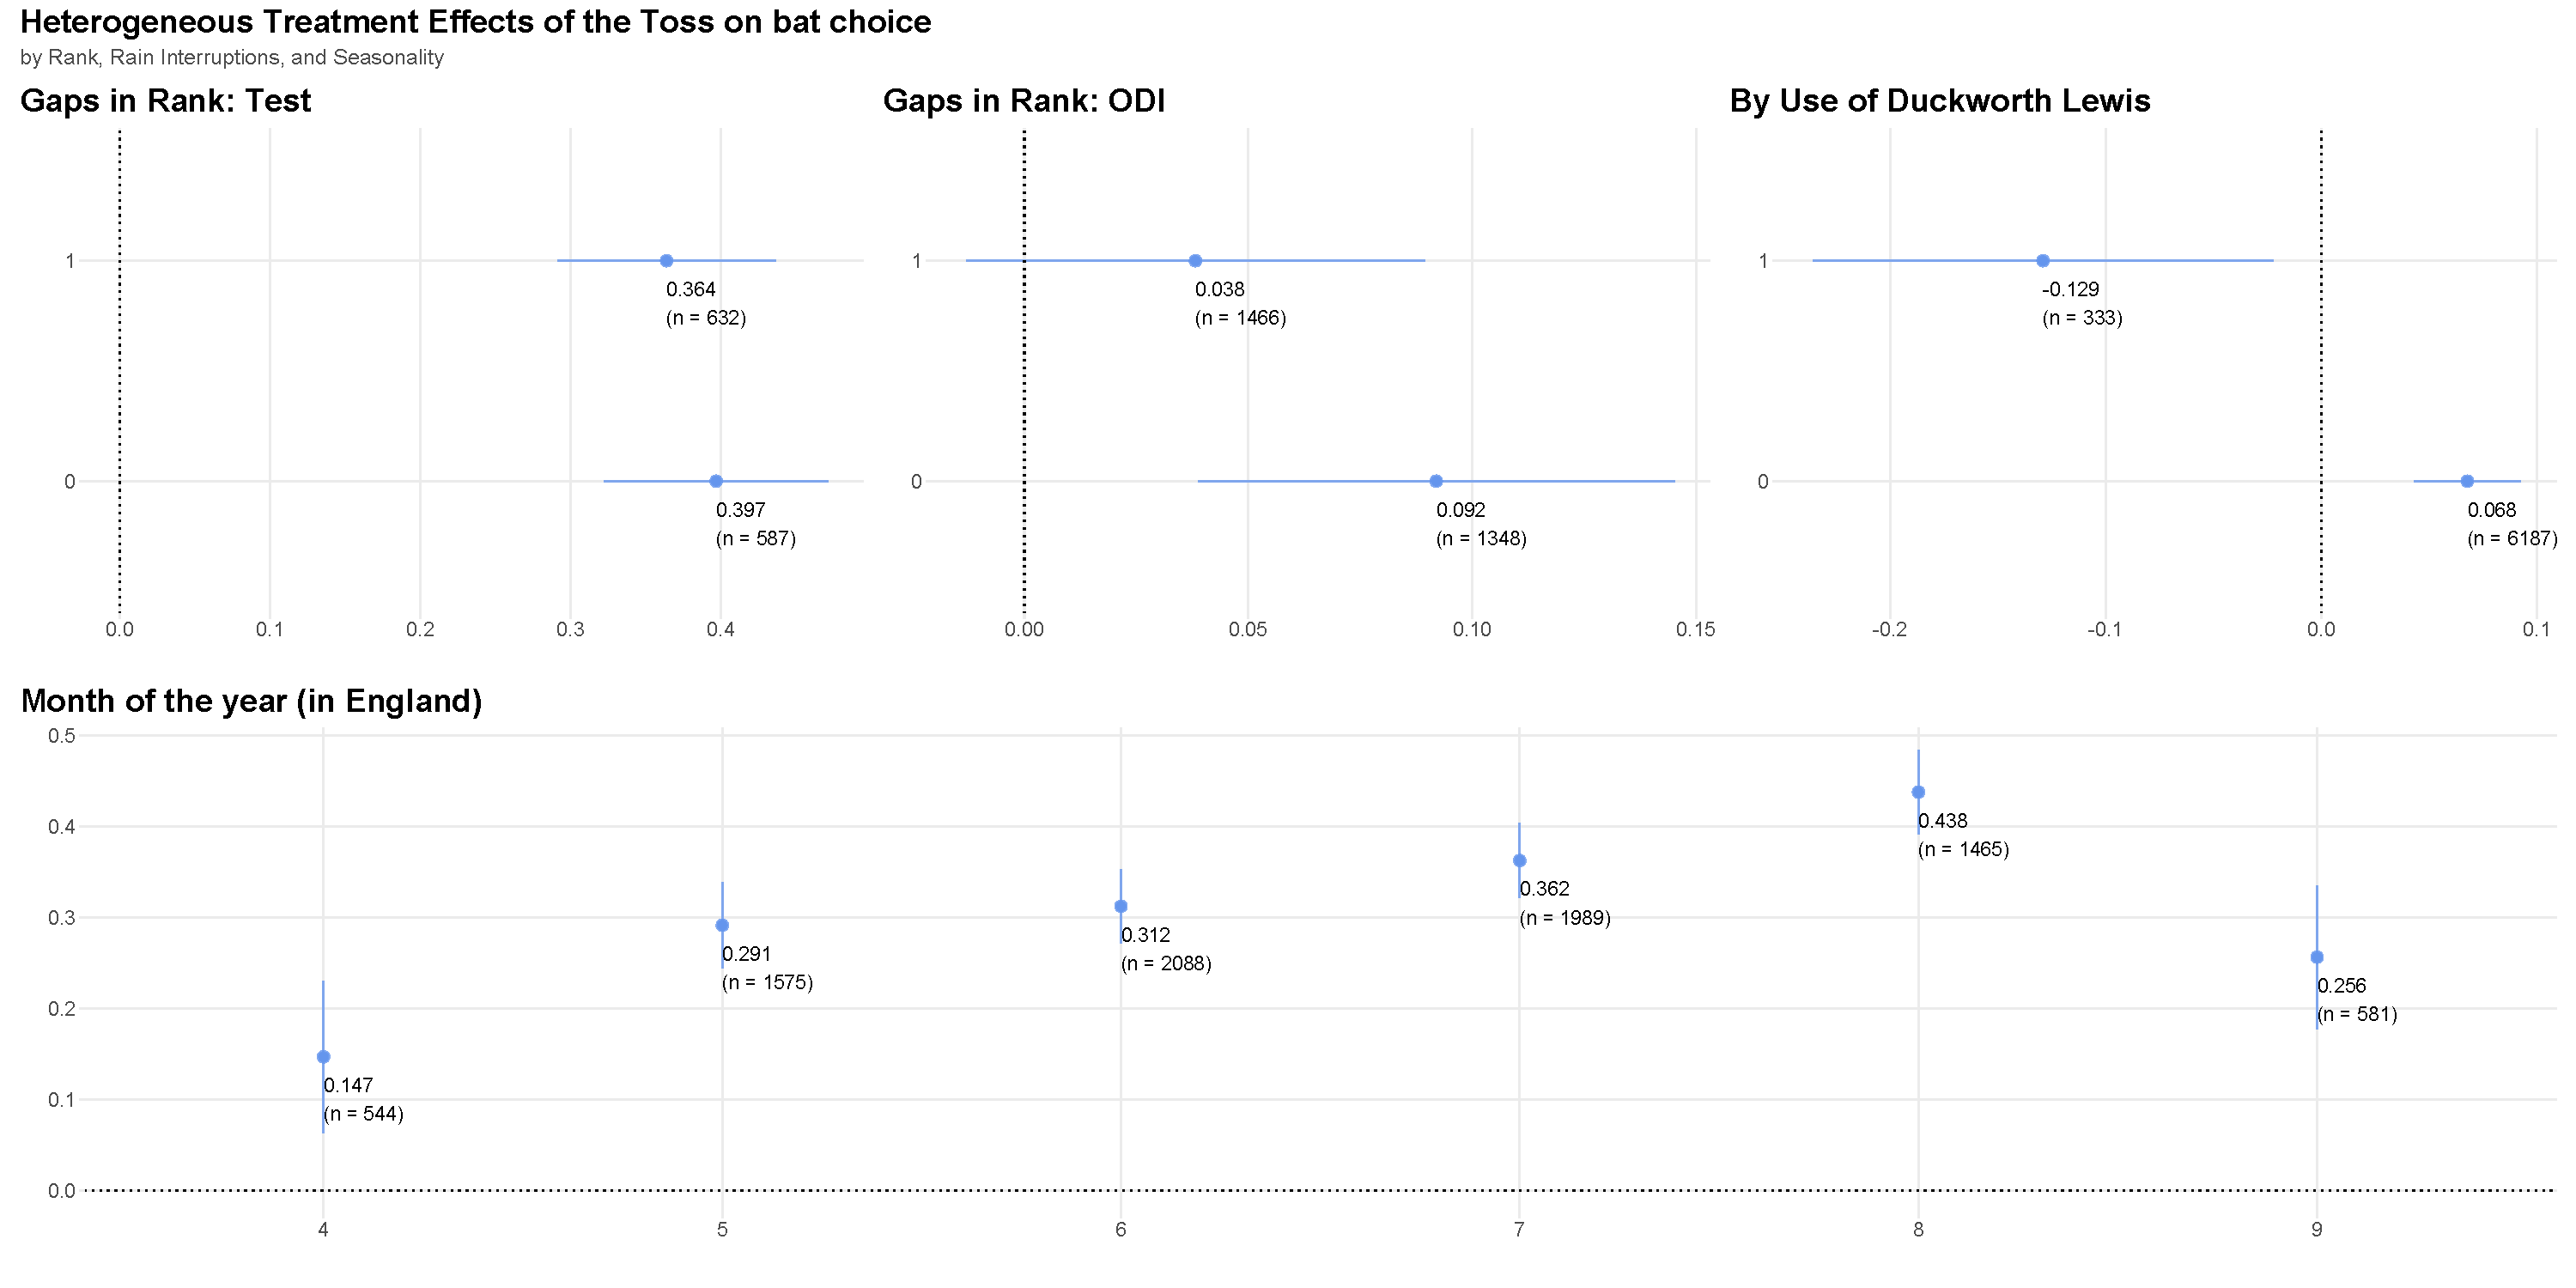
\includegraphics[width=0.9\textwidth,keepaspectratio]{output/first_stage_by_rank_dl_season.pdf}
 \caption{Toss effects on choice to bat decomposed by ranking differences, rain-interruptions, and season (in England)}
 \label{fig:fs_het_TE3}
\end{figure}






\end{document}
